\chapter{The probe}
\label{ch:probe}

The probe is the reason Texture Explorer exists. Given the current material, a texel $(u,v)$, the
shape and the rotation of the solid, and the bump settings, it computes everything that
Chapters~\ref{ch:height} and~\ref{ch:tangent} talk about, and the Inspector panel shows it.

\section{The normal of the bump map}
\code{BumpNormalTangent} implements equation~\eqref{eq:nts}: four bilinear samples one texel
around the point, central differences, and the normal $(-k h_x, -k h_y, 1)$ normalized. It also
returns the slope so that the Inspector can show it.

\excerpt{bumpnormal}

\section{From the texel to the world}
\code{Inspect} first samples every map at the probe. Then it finds the probed texel on the solid
(\code{FindSurfacePoint}), builds the tangent frame there, and multiplies the tangent-space normal
by the TBN matrix. The position is displaced like the vertex shader displaces vertices, so the
arrows start on the surface the user sees. Finally everything is rotated into the world by the
world matrix, which is a pure rotation and therefore also transforms normals correctly
(Section~\ref{sec:normaltransform}).

\excerpt{inspect}

\section{What the Inspector shows}

\begin{figure}[ht]
  \centering
  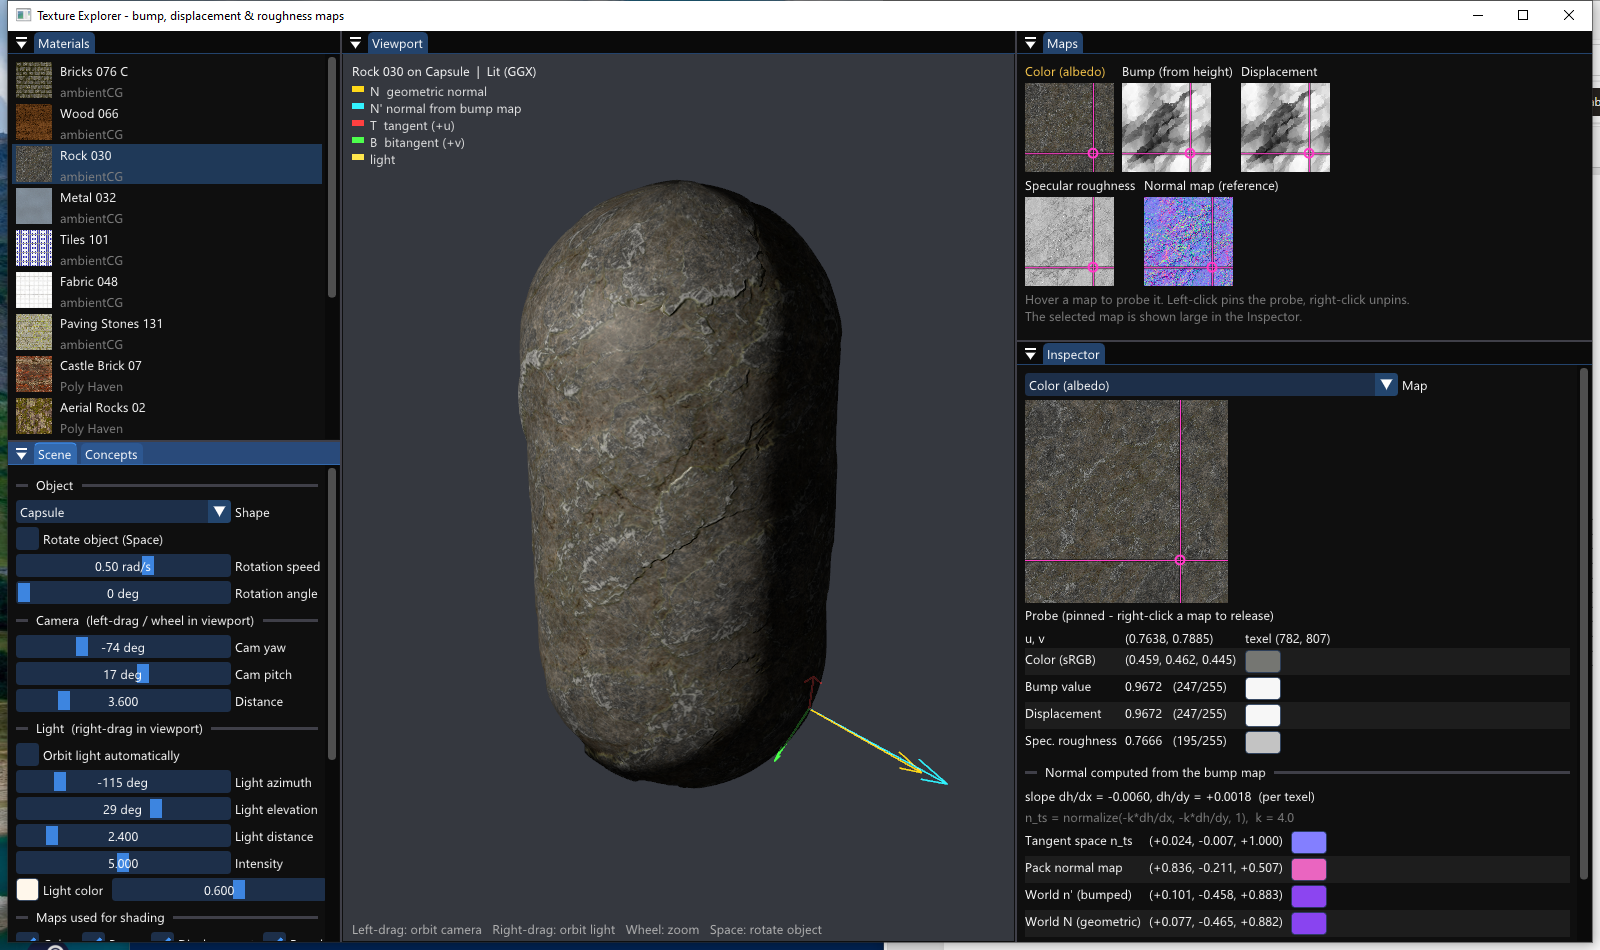
\includegraphics[width=\linewidth]{figures/capsule-roughness.png}
  \caption{The rock material on the capsule, with a pinned probe. Compare the
  ``Tangent space $n_{\mathrm{ts}}$'' row, computed from the bump map, with the ``Pack normal
  map'' row, decoded from the material's own normal map: the material's map was baked from
  much finer geometry, so here it leans far more strongly.}
  \label{fig:capsule}
\end{figure}

The Inspector lists, for the probed texel:
\begin{description}[font=\normalfont\itshape]
\item[u, v] the normalized coordinates and the integer texel;
\item[Color (sRGB)] the stored colour, with a swatch;
\item[Bump value, Displacement, Spec.\ roughness] as fractions and as stored bytes ($/255$);
\item[slope] $h_x$ and $h_y$ in height units per texel;
\item[Tangent space $n_{\mathrm{ts}}$] equation~\eqref{eq:nts}, with its colour encoding
$\frac12\vect n+\frac12$;
\item[Pack normal map] the material's own normal map at the same texel, decoded by
$2\,\mathit{rgb}-1$, for comparison (Section~\ref{sec:normalmaps});
\item[World $\vect n'$, World $\Nv$, World $\Tv$, World $\Bv$, World position] the bumped and the
geometric normals, the frame, and the displaced point, in world coordinates.
\end{description}
The same quantities appear in the 3D view as arrows (Figure~\ref{fig:pyramid}). The bumped normal
$\vect n'$ deviates from $\Nv$ by an angle that grows with the bump strength, and the frame
$\Tv,\Bv$ shows how the texture is laid on the surface at that point.
